% latex

% title: SwipProteomics
% author twab
% description: response to reviewers

\documentclass[12pt]{article}

\usepackage{amsmath}
\usepackage{amssymb}
\usepackage{amsthm}
\usepackage{caption}
\usepackage{changepage}
\usepackage{fancyhdr}
\usepackage{graphicx}
\usepackage{tikz}
\usepackage{titlesec}
\usepackage[margin=1.0in]{geometry}

\graphicspath{ {./figs/} }

%\usepackage[T1]{fontenc}
\usepackage{inconsolata}


\pagestyle{fancy}

\lhead{Tyler W. A. Bradshaw}
\rhead{Response to eLife Reviewers} 

\setlength\parindent{0pt}
\pagenumbering{gobble} 
% options includearabic, roman, Roman, alph, Alph, gobble--supress numbering

\begin{document}

At the centre of the reviewers' cogent critique of our manuscript 
was the questioned statistical validity of our approach. Succinctly, 
the issue at question is whether or not the R package \texttt{edgeR}
is an appropriate tool for analysis of protein mass spectrometry data.\\

High level statistical inference in \texttt{edgeR} is built on a 
negative binomial (NB) generalized linear model (GLM) framework. 
The data are assumed to be adequately described by a NB distribution 
parameterized by a dispersion parameter, $\phi$. \footnotemark \\

\footnotetext{ The dispersion parameter can take several forms. 
p supports three types of dispersion models: 'common', 'trended', and
'tagwise'. When using \texttt{edgeR's} robust quasi-likelihood test methods, 
only global (i.e. 'common' or 'trended') dispersions are appropriate 
(see ?\texttt{edgeR::glmQLFit}).}

Our previous approach used a customized workflow\footnotemark, to preprocessing
and normalize the data. We used \texttt{edgeR} to perform statistical testing  
using its flexible GLM framework.

\footnotetext{ The most important step in our normalization approach is 
IRS normalization. IRS normalization scales protein measurements using an 
internal reference standard to normalize protein measurments between TMT MS
runs. This is essential to account for the stochasticisity of peptide
quantification in MS experiments. Phillip Wilmarth's GitHub offers an 
excellent exploration of IRS normalization.
}

Our decision to use \texttt{edgeR} was motivated by numerous 
conceptual and practical considerations. \texttt{edgeR} is an excellent package,
and should be strongly considered when analyzing RNA-sequencing data. Here we 
only consider its appropriatness for our TMT dataset.

\begin{figure}[!h]
	%\begin{center}
		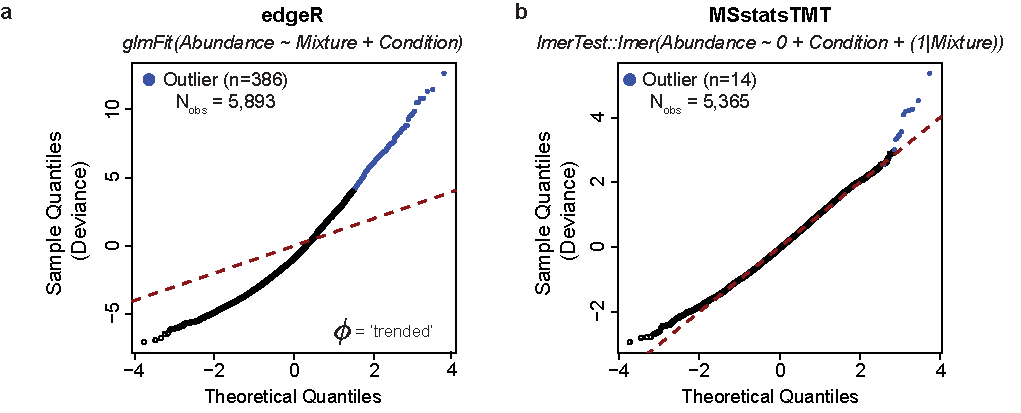
\includegraphics{fig_01}
		\caption{\textbf{Goodness-of-fit of \texttt{edgeR} (A), and 
		\texttt{MSstats} (B) statistical approaches.} The overall
		adequacy of the models were assessed using a quantile-quantile
		plot (McCarthy et al (2012)). \textbf{(A)} The normalized
		protein data were fit with a fixed effects model of the form: 
		\texttt{Abundance ~ Mixture + Condition}
		Outliers indicate proteins with poor fits.
		Where \texttt{Mixure} 
		is a blocking factor to accound for batch effects between
		experiments. The residual deviance for all proteins is plotted as
		a  quantile-quantile (QQ) plot using \texttt{edgeR::gof}.
		\textbf{(B)}
		The normalized protein data were fit with a linear mixed-effects 
		model of the formand the residual deviance and degrees of 
		freedom extracted from the fitted models. The z-normalized
		deviance were plotted as in (A). The QQ-plot shows that the
		residual deviance is normally distributed.}
	%\end{center}
\end{figure}

\end{document}
